\chapter{Background}

\section{Graph Theoretic Notations}

\section{LLVM Compiler Infrastructure}

LLVM was originally proposed as a \textit{Low-Level Virtual Machine}\footnote{Although LLVM was initially an acronym for Low-Level Virtual Machine, it is now a brand that applies to the whole LLVM umbrella project.}, extending previous work on virtual instruction set architectures~\citep{adve03,lattner04}.
Since then, LLVM has evolved into an umbrella project that comprises a collection of modular and reusable compiler and toolchain technologies.
The main components under the LLVM umbrella is the LLVM intermediate representation (IR) and the LLVM \textit{Core} libraries.

The LLVM compiler infrastructure implements the classical \textit{three-phase compiler} infrastructure, which consists of a frontend, an optimiser, and a backend.
The frontend is responsible for parsing, validating and diagnosing errors in the source code.
This parsed source code is then translated into an intermediate representation, which is the LLVM IR in this case.
The optimiser is responsible for doing a broad variety of transformations, that are usually independent of language and target machine, to improve the code's performance.
%The front end parses source code, checking it for errors, and builds a language-specific Abstract Syntax Tree (AST) to represent the input code. The AST is optionally converted to a new representation for optimization, and the optimizer and back end are run on the code.
%The optimizer is responsible for doing a broad variety of transformations to try to improve the code's running time, such as eliminating redundant computations, and is usually more or less independent of language and target.
The backend, also known as the code generator, then translates the code from the intermediate representation onto the target instruction set.
It is common for the backend to also perform some low-level optimisations that take advantage of unusual features of the supported architecture.
%Common parts of a compiler backend include instruction selection, register allocation, and instruction scheduling.

\begin{figure}[h]
  \centering
  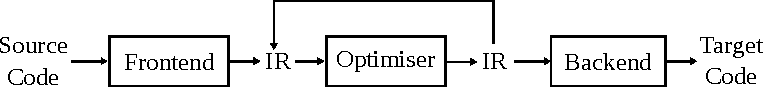
\includegraphics[scale=0.9]{figs/3-phase-compiler.pdf}
  \caption{Overview of the three-phase compiler infrastructure.}
  \label{fig:3-phase-compiler}
\end{figure}

%This IR is optionally fed through a series of analysis and optimization passes which improve the code, then is sent into a code generator to produce native machine code, as shown in Figure 11.3.
%This is a very straightforward implementation of the three-phase design, but this simple description glosses over some of the power and flexibility that the LLVM architecture derives from LLVM IR.

%The most important aspect of its design is the LLVM Intermediate Representation (IR), which is the form it uses to represent code in the compiler.
%LLVM IR is designed to host mid-level analyses and transformations that you find in the optimizer section of a compiler.
%It was designed with many specific goals in mind, including supporting lightweight runtime optimizations, interprocedural optimizations, whole program analysis, and aggressive restructuring transformations, etc.

%Like a real RISC instruction set, it supports linear sequences of simple instructions like add, subtract, compare, and branch.

\subsection{LLVM Virtual Instruction Set}

LLVM IR is a low-level RISC-like virtual instruction set.
It differs from other intermediate representations (e.g. GCC's GENERICS or the most recent GCC's GIMPLE) as it is defined as a first class language with well-defined semantics.
Beyond being implemented as a language, LLVM IR is actually defined in three isomorphic forms: the textual format above, an in-memory data structure inspected and modified by optimizations themselves, and an efficient and dense on-disk binary \textit{bitcode} format.
%The LLVM Project also provides tools to convert the on-disk format from text to binary: llvm-as assembles the textual .ll file into a .bc file containing the bitcode goop and llvm-dis turns a .bc file into a .ll file.

Unlike most RISC instruction sets, LLVM is strongly typed with a simple language-independent type system.
LLVM's type system can be used to implement data types and operations from high-level languages exposing their implementation behaviour to all stages of optimisation.
This type system includes the type information used by sophisticated techniques, such as algorithms for pointer analysis, dependence analysis, and data transformations.
LLVM also offers instructions for performing type conversions and low-level address arithmetic while preserving type information.
Furthermore, LLVM IR also differs from RISC instruction sets as some details of the machine are abstracted away.
For example, the calling convention is abstracted through call and ret instructions and explicit arguments.
Another significant difference from machine code is that the LLVM IR has an infinite set of virtual registers (which are named with a \% character), insted of having just a fixed set of named registers.

The LLVM type system is considered one of the most important features of its intermediate representation, as it enables several optimisations to be performed directly on the IR, without having to do extra analyses on the side before the transformation.
The main first class types supported are: single value types, aggregate types, and labels.
Single value types consist of integers of arbitrary bit width (e.g.\lstinline[language=llvm,style=nasm]{i32} denotes a 32-bit integer), floating-point of commonly used width (e.g.\lstinline[language=llvm,style=nasm]{half},\lstinline[language=llvm,style=nasm]{float},\lstinline[language=llvm,style=nasm]{double}, and\lstinline[language=llvm,style=nasm]{fp128}), pointers (e.g.\lstinline[language=llvm,style=nasm]{i32*}) and vector types.
Vectors are used when multiple primitive data are operated in parallel using a single instruction (SIMD).
A vector type is represented by a the number of elements and an underlying primitive data type, e.g.\lstinline[language=llvm,style=nasm]{<4 x i32>} is a vector of four 32-bit integer values.
Aggregated types consist of arrays and structures.
Vectors are not considered to be aggregate types.

In addition to type information, LLVM IR also provides other high-level information that are useful for effectively performing several code analysis and transformations.
This includes explicit control flow graphs (CFG)~\citep{allen70} and an explicit dataflow representation, by means of the infinite register set in \textit{static single assignment} (SSA) form~\citep{alpern88,cytron89,cytron91}.

A control flow graph (CFG) is a directed graph in which the nodes represent basic blocks and the edges represent control flow paths, i.e. edges represent transfers of control (jumps) between basic blocks.
A basic block is a straight-line sequence of instructions having only one entry point, i.e. the first instruction to be executed in the basic block, and only one exit point, i.e. the last instruction executed~\citep{allen70,cytron91}.
Figure~\ref{fig:cfg-odd_inc} shows an example of a CFG constructed from the code in Listing~\ref{lst:ex:odd_inc}.

An IR is in SSA form if and only if each virtual register is assigned exactly once and every use of registers occur after their definition.
The primary advantage of using the SSA form is that it simultaneously simplifies and improves several compiler optimisations and analysis~\citep{alpern88,cytron91}.
Most of the industrial-strength compilers for imperative programming language rely heavily on the SSA form.

\begin{lstlisting}[language=llvm,style=nasm,caption={An illustrative example of a function in textual LLVM IR. This function returns the argument incremented by one if it is even or by two if it is an odd integer.}, label={lst:ex:odd_inc}]
define i32 @odd_inc(i32 %arg) {
entry:
  %rem = srem i32 %arg, 2
  %cmp = icmp eq i32 %rem, 0
  br i1 %cmp, label %if.then, label %if.else
if.then:
  %add.1 = add i32 %arg, 1
  br label %if.end
if.else:
  %add.2 = add i32 %arg, 2
  br label %if.end
if.end:
  %ans = phi i32 [ %add.1, %if.then ], [ %add.2, %if.else ] [!\label{lst:odd_inc:phi}!]
  ret i32 %ans
}
\end{lstlisting}

Listing~\ref{lst:ex:odd_inc} shows an example of a function written using textual LLVM IR.
Names starting with the @ character have a global scope, while names starting with \% have a local scope.
As stated previously, LLVM IR is strongly typed, which means that every virtual register is attributed a specific type (e.g.\lstinline[language=llvm,style=nasm]{i32 %arg} is of type\lstinline[language=llvm,style=nasm]{i32}, namely a 32-bit integer) as well as every operation (e.g.\lstinline[language=llvm,style=nasm]{add i32} expects all operands of type\lstinline[language=llvm,style=nasm]{i32}).
Instructions use the three address format, which refers to the use of three operands by most of the instructions.
However, instructions with fewer or more operands may occur, e.g. the\lstinline[language=llvm,style=nasm]{ret} instruction have fewer operands, while the\lstinline[language=llvm,style=nasm]{phi} and the\lstinline[language=llvm,style=nasm]{call} instructions may have more than three operands.

Furthermore, the SSA form requires a special assignment statements called the $\phi$-function (see line \ref{lst:odd_inc:phi} of Listing~\ref{lst:ex:odd_inc}).
The $\phi$-function receives as argument a list of virtual registers from different  control flow predecessors of the point where the $\phi$-function occurs.
The control flow predecessors of each point in the CFG are listed in some arbitrary fixed order, and the $i$-th operand of $\phi$-function is associated with the $i$-th predecessor.
If control reaches the $\phi$-function from its $i$-th predecessor, then the value of the $i$-th operand is attributed in the assignment.
Each execution of a $\phi$-function uses only one of the operands, but which one depends on the flow of control just before the $\phi$-function.

\begin{figure}[h]
  \centering
  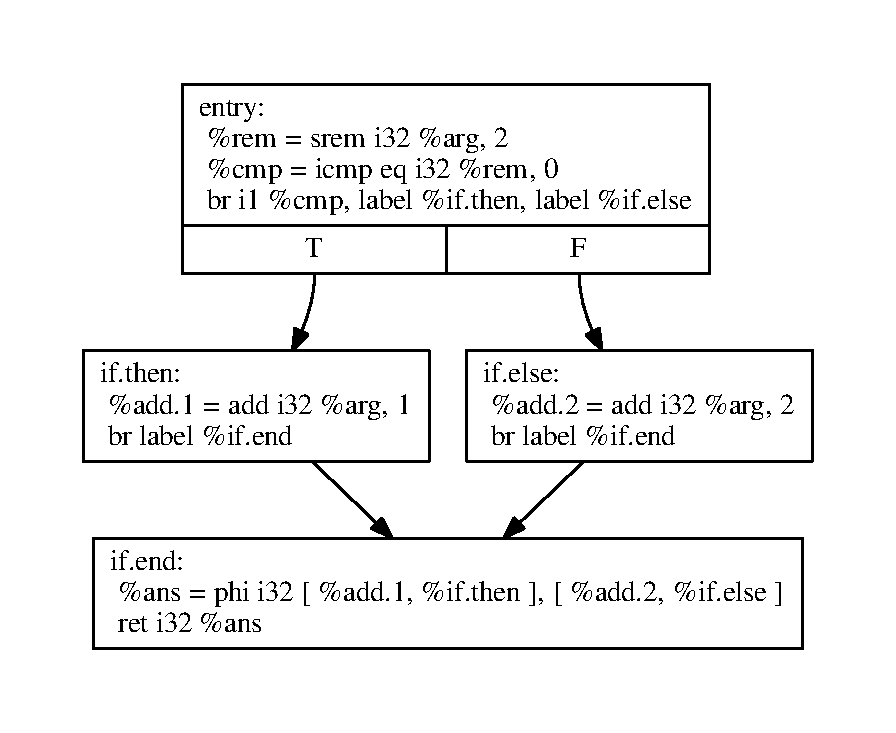
\includegraphics[scale=0.7]{figs/cfg-odd_inc.pdf}
  \caption{Control flow graph of the\lstinline[language=llvm,style=nasm]{odd_inc} function (see Listing~\ref{lst:ex:odd_inc}).}
  \label{fig:cfg-odd_inc}
\end{figure}

In addition to virtual registers, LLVM also allows for stack allocated local variables.
These are created by allocating data on the stack frame of the currently executing function.
Data from the stack frame can be manipulated by using explicit memory access operations.
Figure~\ref{lst:ex:odd_inc_stack} shows an implementation of the\lstinline[language=llvm,style=nasm]{odd_inc} function using data allocated on the stack frame.
This implementation avoids using the $\phi$-function by keeping the answer on the stack.

LLVM provides an optimisation pass for promoting memory references to be register references (called \texttt{-mem2reg}).
It promotes alloca instructions which only have loads and stores as uses.
An alloca is transformed by using dominator frontiers to place phi nodes, then traversing the function in depth-first order to rewrite loads and stores as appropriate.

\begin{lstlisting}[language=llvm,style=nasm,caption={An example of the odd\_inc function implemented using data allocated on the stack frame.}, label={lst:ex:odd_inc_stack}]
define i32 @odd_inc_stack(i32 %arg) {
entry:
  %addr = alloca i32
  %rem = srem i32 %arg, 2
  %cmp = icmp eq i32 %rem, 0
  br i1 %cmp, label %if.then, label %if.else
if.then:
  %add.1 = add i32 %arg, 1
  store i32 %add.1, i32* %addr
  br label %if.end
if.else:
  %add.2 = add i32 %arg, 2
  store i32 %add.2, i32* %addr
  br label %if.end
if.end:
  %ans = load i32, i32* %addr
  ret i32 %ans
}
\end{lstlisting}

%\textbf{Another difference between LLVM and GCC:}

%In particular, LLVM IR is both well specified and the only interface to the optimizer.
%This property means that all you need to know to write a front end for LLVM is what LLVM IR is, how it works, and the invariants it expects.
%Since LLVM IR has a first-class textual form, it is both possible and reasonable to build a front end that outputs LLVM IR as text, then uses Unix pipes to send it through the optimizer sequence and code generator of your choice.

%It might be surprising, but this is actually a pretty novel property to LLVM and one of the major reasons for its success in a broad range of different applications.
%Even the widely successful and relatively well-architected GCC compiler does not have this property: its GIMPLE mid-level representation is not a self-contained representation.
%As a simple example, when the GCC code generator goes to emit DWARF debug information, it reaches back and walks the source level "tree" form.
%GIMPLE itself uses a "tuple" representation for the operations in the code, but (at least as of GCC 4.5) still represents operands as references back to the source level tree form.

%The implications of this are that front-end authors need to know and produce GCC's tree data structures as well as GIMPLE to write a GCC front end.
%The GCC back end has similar problems, so they also need to know bits and pieces of how the RTL back end works as well.
%Finally, GCC doesn't have a way to dump out "everything representing my code", or a way to read and write GIMPLE (and the related data structures that form the representation of the code) in text form. The result is that it is relatively hard to experiment with GCC, and therefore it has relatively few front ends.

\subsection{Analysis and Transformation Passes}

The LLVM Pass Framework is an important part of the LLVM system, because LLVM passes are where most of the interesting parts of the compiler exist.
Passes perform the transformations and optimizations that make up the compiler, they build the analysis results that are used by these transformations, and they are, above all, a structuring technique for compiler code.

\begin{figure}[h]
  \centering
  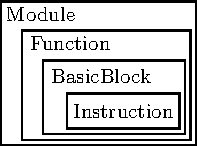
\includegraphics[scale=1]{figs/llvm-containers.pdf}
  \caption{.}
  \label{fig:llvm-containers}
\end{figure}


\section{Early Work in {\IterComp}}

\textbf{Original work in {\IterComp}: single input and offline}

\section{Program Profiling}

\textbf{Basic background about profiling in general}

\section{Summary}
